\section{Latex 图形绘制宏包}
\subsection{树状结构图 dirtree}
\subsubsection{dirtree 代码}
\index{宏包!dirtree}
\index{命令!\verb$\dirtree$}
使用 dirtree 宏包。如下图所示

\dirtree{%
.1 /.
.2 bin.
.2 home.
.3 jeancome.
.4 texmf.
.5 tex.
.6 latex.
.7 dirtree.
.3 jeancomeson.
.3 jeancomedaughter.
.2 usr.
.3 bin.
.3 games.
.4 fortunes.
.3 include.
.3 local.
.4 bin.
.4 share.
.5 texmf.
.6 fonts.
.6 metapost.
.6 tex.
.3 share.
}
对应代码如下:
\begin{lstlisting}
\dirtree{%
.1 /.
.2 bin.
.2 home.
.3 jeancome.
.4 texmf.
.5 tex.
.6 latex.
.7 dirtree.
.3 jeancomeson.
.3 jeancomedaughter.
.2 usr.
.3 bin.
.3 games.
.4 fortunes.
.3 include.
.3 local.
.4 bin.
.4 share.
.5 texmf.
.6 fonts.
.6 metapost.
.6 tex.
.3 share.
}
\end{lstlisting}




\subsubsection{dirtree 参数设计}
\begin{description}
  \item[DTstyle] 结点文字的属性
  \item[DTcomment] 右侧注释的内容
  \item[DTstylecomment] 右侧注释文字的属性
  \item[DTsetlength] 如下图所示
\begin{figure}[H]
  \centering
  % Requires \usepackage{graphicx}
  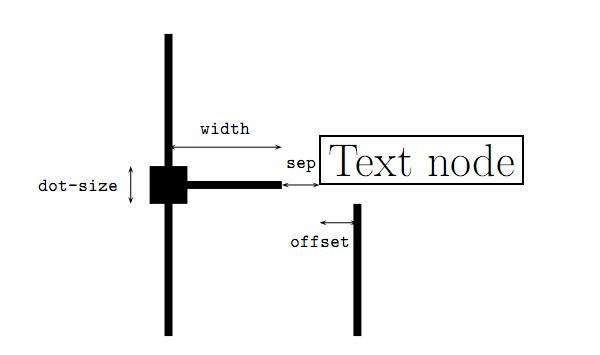
\includegraphics[width=10cm]{dirtree_length}\\
  \caption{dirtree 长度设置}\label{dirtree_length}
\end{figure}

\begin{cmd}[label= 长度设置命令]
    \DTsetlength{offset}{width}{sep}{rule-width}{dot-size}
默认值如下:
• offset=0.2em
• width=1em
• sep=0.2em
• rule-width=0.4pt
• dot-size=1.6pt
\end{cmd}
  \item[DTbaselineskip] 基线设置

\begin{cmd}[label= 基线设置命令]
\setlength{\DTbaselineskip}{20pt}
\DTsetlength{1em}{3em}{0.1em}{1pt}{4pt}
\end{cmd}
\end{description}

\renewcommand*\DTstylecomment{\rmfamily\color{green}\textsc}
\renewcommand*\DTstyle{\ttfamily\textcolor{red}}
\dirtree{%
.1 /.
.2 bin.
.2 home.
.3 jeancome.
.4 texmf.
.5 tex.
.3 jeancomeson\DTcomment{Guillaume}.
.3 jeancomedaughter\DTcomment{Mathilde}.
.2 usr.
.3 bin.
}


\lstset{language=[LaTeX]TeX}
\begin{lstlisting}
\dirtree{%
.1 /.
.2 bin.
.2 home.
.3 jeancome.
.4 texmf.
.5 tex.
.3 jeancomeson\DTcomment{Guillaume}.
.3 jeancomedaughter\DTcomment{Mathilde}.
.2 usr.
.3 bin.
}
\end{lstlisting}


\dirtree{%
.1 /.
.2 bin\ldots{}\begin{minipage}[t]{5cm}
This directory hold sexecutable files (binary
files or link on binary files){.}
\end{minipage}.
.2 home\ldots{}\begin{minipage}[t]{5cm}
jeancome\\
guillaume\\
mathilde\\
\end{minipage}.
.4 texmf.
}

\begin{lstlisting}

\dirtree{%
.1 /.
.2 bin\ldots{}\begin{minipage}[t]{5cm}
This directory hold sexecutable files (binary
files or link on binary files){.}
\end{minipage}.
.2 home\ldots{}\begin{minipage}[t]{5cm}
jeancome\\
guillaume\\
mathilde\\
\end{minipage}.
.4 texmf.
}
\end{lstlisting}

\subsection{栈的绘制 drawstack}

\subsubsection{Minimalistic example}

% The main feature of the package is to define an environment
% drawstack.
\begin{drawstack}
  % Within the environment, draw stack elements with \cell{...}
  \cell{First cell}
  \cell{Second cell}
\end{drawstack}

\subsubsection{Grouping cells into stack frames}

\begin{drawstack}
  \startframe
  \cell{First cell}
  \cell{Second cell}
  \finishframe{Some stack frame}
  \cell{Not interesting}
  \startframe
  \cell{Next stack frame}
  \cell{Next stack frame}
  \finishframe{Another stack frame}
\end{drawstack}

\subsubsection{Stack and Base pointers}

\begin{drawstack}
  \startframe
  % \cellcom writes something on the right-hand side of a cell.
  \cell{loc2} \cellcom{-8(\%ebp)}
  \cell{loc1} \cellcom{-4(\%ebp)}
  % \esp and \ebp are stack pointer and base pointer in Pentium.
  % These macros are simple shortcuts for \cellptr{...}
  \cell{Sauvegarde \%ebp} \esp \ebp
  \cell{@ retour} \cellcom{4(\%ebp)}
  \finishframe{fonction\\ {\tt f}}
  \startframe
  \cell{} \cellcom{8(\%ebp)}
  \cell{}
  \finishframe{fonction\\ {\tt main}}
\end{drawstack}

\subsubsection{Padding}

\begin{drawstack}
  \cell{above padding}
  \padding{3}{nothing here}
  \cell{below padding}
\end{drawstack}

\subsubsection{Below/Above stack pointer}

\begin{drawstack}
  \cell{Top}
  \cell{Below top}
  % \bcell is just like \cell, but in a different color.
  \bcell{Above bottom} \cellptr{Stack pointer here}
  \bcell{Bottom}
\end{drawstack}

\subsubsection{Highlighting some cell}

\begin{drawstack}
  \cell{Uninteresting cell}
  \cell{Interesting cell} \cellround{Yes, this one!}
\end{drawstack}

\subsubsection{Using tikzpicture instead of drawstack}

% The environment drawstack is basically a syntactic sugar for
%
% \begin{tikzpicture}[#1]
% \stacktop{}
% ...
% \stackbottom
% \end{tikzpicture}
%
% You can use the above syntax for more flexibility.

\begin{tikzpicture}[scale=0.8]
  \small
  \stacktop{}
  \cell{My cell}
  \stackbottom{}
\end{tikzpicture}

\subsubsection{Changing style}

{% tikzstyle will be local to this {...}
\tikzstyle{freecell}=[fill=blue!10,draw=blue!30!black]
\tikzstyle{occupiedcell}=[fill=blue!10!orange!10,draw=blue!30!black]
\tikzstyle{padding}=[fill=yellow!20,draw=blue!30!black]
\tikzstyle{highlight}=[draw=orange!50!black,text=orange!50!black]

\begin{drawstack}
  \cell{Uninteresting cell}
  \cell{Interesting cell} \cellround{Yes, this one!}
  \bcell{bcell}
  \padding{2}{Padding}
\end{drawstack}
}

\subsubsection{Example: Computing Factorial}

\begin{drawstack}[scale=0.8]
  \startframe
  \cell{N = 1}
  \cell{...}
  \finishframe{fact(1)}
  \startframe
  \cell{N = 2}
  \cell{...}
  \finishframe{fact(2)}
  \cell{$\vdots$}
  \startframe
  \cell{N = 5}
  \cell{...}
  \finishframe{fact(5)}
\end{drawstack}

\subsection{柱状图 bardiag}
\index{宏包!bardiag}
\index{命令!\verb$\bardiag$}
\index{命令!\verb$\betweenticks$}
\subsubsection{bardiag 代码}
\renewcommand{\betweenticks}{50}
\bardiagrambegin{9.5}{200}{2cm}{1}{2}{1cm}{0.05cm}
\drawlevellines
\baritem{1998}{120}{green}
\baritem{1999}{123}{red}
\baritem{2000}{147}{yellow}
\baritem{2001}{176}{green}
\baritem{2002}{132}{red}
\bardiagramend{{\large Year}}{{\large Income}}

\lstset{language={[LaTeX]TeX}}
\begin{lstlisting}
\renewcommand{\betweenticks}{50}
\bardiagrambegin{9.5}{200}{2cm}{1}{2}{1cm}{0.05cm}
\drawlevellines
\baritem{1998}{120}{green}
\baritem{1999}{123}{red}
\baritem{2000}{147}{yellow}
\baritem{2001}{176}{green}
\baritem{2002}{132}{red}
\bardiagramend{{\large Year}}{{\large Income}}
\end{lstlisting}

\subsubsection{bardiag 参数设计}
\begin{figure}[H]
  \centering
  % Requires \usepackage{graphicx}
  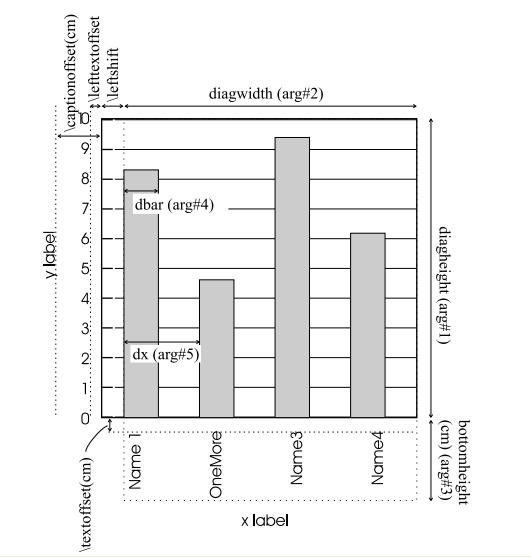
\includegraphics[width=14cm]{bardiag_set}\\
  \caption{bardiag 参数设计}\label{bardiag_set}
\end{figure}